\chapter{Implémentations et synthèse de texture}
\label{chap:chapitre2}

Notre recherche est une étude exploratoire du modèle multi-résolutionnel local, en particulier de la PC, issu du traitement d'image, appliquée dans le contexte de la synthèse de texture. Nous allons maintenant voir la mise en application des concepts exposés à la partie précédente, ainsi que les résultats obtenus.

\section{Implémentation}

% todo formu négative a eviter
Les concepts d'énergie locale et de signal monogène ne sont pas des notions communément utilisées dans le traitement d'image, aucune librairie standard ne les implémente à notre connaissance. Nous avons donc dû implémenter nous-même les algorithmes pour mettre en place le modèle multi-résolutionnel local. Le choix du logiciel pour faire ces implémentations a été une question importante.


\paragraph{OpenCV}

Malgré notre but final de travailler sur de la synthèse de texture, nous avons commencé par développer un petit logiciel pour pouvoir itérer rapidement et expérimenter avec les concepts de base du modèle multi-résolutionnel local sur des images, sans prendre en compte les problématiques de la synthèse. Pour cela, nous mis au point un logiciel utilisant \cpp avec la librairie OpenCV~\cite{opencv_library}. OpenCV est une librairie standard de traitement d'image en temps réel et de vision par ordinateur, disponible pour les langages de programmation \cpp, Python et Java. Les images y sont représentées comme des matrices, et les opérations de bas niveau courantes du traitement d'image y sont implémentées, comme la lecture, l'écriture, l'affichage, le filtrage, la convolution, et autres. Notre logiciel permet à un utilisateur de créer, visualiser, et modifier les pyramides d'une image d'entrée, ainsi que de calculer et visualiser la PC. Avec ces fonctionnalités, nous avons fait des expérimentations pour voir l'effet de différentes modifications et reconstructions de la pyramide de Riesz d'une image.

\bigskip

Plusieurs raisons ont ensuite motivé notre choix de changer d'implémentation. Après avoir expérimenté avec la PC sur des images, nous voulions travailler avec des textures, c'est-à-dire faire de la synthèse dans le cadre du \textit{pipeline graphique} traditionnel. Plus que simplement reconstruire une image, nous souhaitions maintenant synthétiser une texture à projeter sur une surface, potentiellement infinie, dans le but de la recouvrir. Dans un tel contexte, plusieurs problématiques surviennent. La synthèse de texture doit pouvoir se faire dans le \textit{fragment shader}, depuis le GPU, pour être mise en place dans le \textit{pipeline graphique}. Cela veut dire avoir une méthode de reconstruction parallélisable, ce qui n'est pas le cas de la méthode que nous utilisions jusque-là. Se posent aussi des questions de projection et de filtrage, que n'avions pas eu à traiter jusque-là, mais nécessaires à considérer pour de la synthèse de texture.

\bigskip

Parallèlement, notre laboratoire de recherche a accueilli de nouveaux membres, qui travaillaient sur des problématiques similaires aux nôtres. Nous voulions alors mettre en place un logiciel qui servirait de base de travail commune pour les personnes faisant de la synthèse de texture dans le laboratoire. Nous avons considéré plusieurs options, notamment développer un moteur de rendu personnalisé et adapté à nos besoins, ou utiliser un des moteurs de jeu Unity3D~\cite{unity_engine} ou Unreal Engine~\cite{unreal_engine}. Le problème d'un moteur personnalisé est qu'il nous aurait fallu réimplémenter beaucoup de choses nous-même, ce qui aurait été long et redondant. Les moteurs Unity3D et Unreal Engine, eux, avaient le désavantage de ne pas offrir la flexibilité de manipuler les textures tel que nous souhaitions le faire. Nous avons donc choisi une autre option, le moteur de jeu Godot~\cite{godot_game_engine}.

\paragraph{Godot}

Godot est un logiciel libre et gratuit, moteur de jeu 2D et 3D, qui permet de faire du rendu temps-réel et donc de s'intéresser aux problématiques de la synthèse de texture, ce que ne permettait pas OpenCV. Bien que pour l'instant moins populaire que Unity et Unreal Engine, Godot est une solution qui croit en notoriété, surtout dans la recherche en informatique graphique, car il est léger et flexible, et permet facilement d'écrire des modules personnalisés ou de modifier du code source pour s'adapter aux besoins des utilisateurs. C'est ce que nous avons fait avec Nicolas Lutz, postdoctorant du laboratoire. Nous avons travaillé conjointement à développer \textit{TexSyn}, une librairie \cpp de traitement d'image et de synthèse de texture pour Godot.
%TODO justifier un peu plus godot

\bigskip

Godot a une classe qui gère les textures, mais la manipuler est compliqué et peu efficace pour des opérations d'accès direct dont nous avons besoin pour nos synthèses. Notre librairie \textit{TexSyn} définit une classe d'image plus pratique à utiliser, avec toutes les opérations dont nous avons besoin, qui est ensuite interfacée avec la classe d'image de Godot pour être utilisée depuis l'éditeur. On construit SY avec cela nos pyramides en pré-calcul sur le CPU, que l'on stocke dans des atlas de textures, qui sont ensuite chargés sur le GPU. On fait alors la reconstruction depuis nos \textit{shaders}, en temps réel, en utilisant les pyramides stockées dans les atlas. Cette reconstruction a cependant des problèmes de filtrage, car nous ne pouvons pas appliquer de convolution avec un filtre pour faire un lissage depuis le \textit{fragment shader}. Nous avons ensuite travaillé à développer une méthode de synthèse pouvant traiter des textures à structure irrégulière, en mettant au point un échantillonneur préservant la PC, détaillé plus loin dans ce chapitre.

\begin{figure}
    \centering
    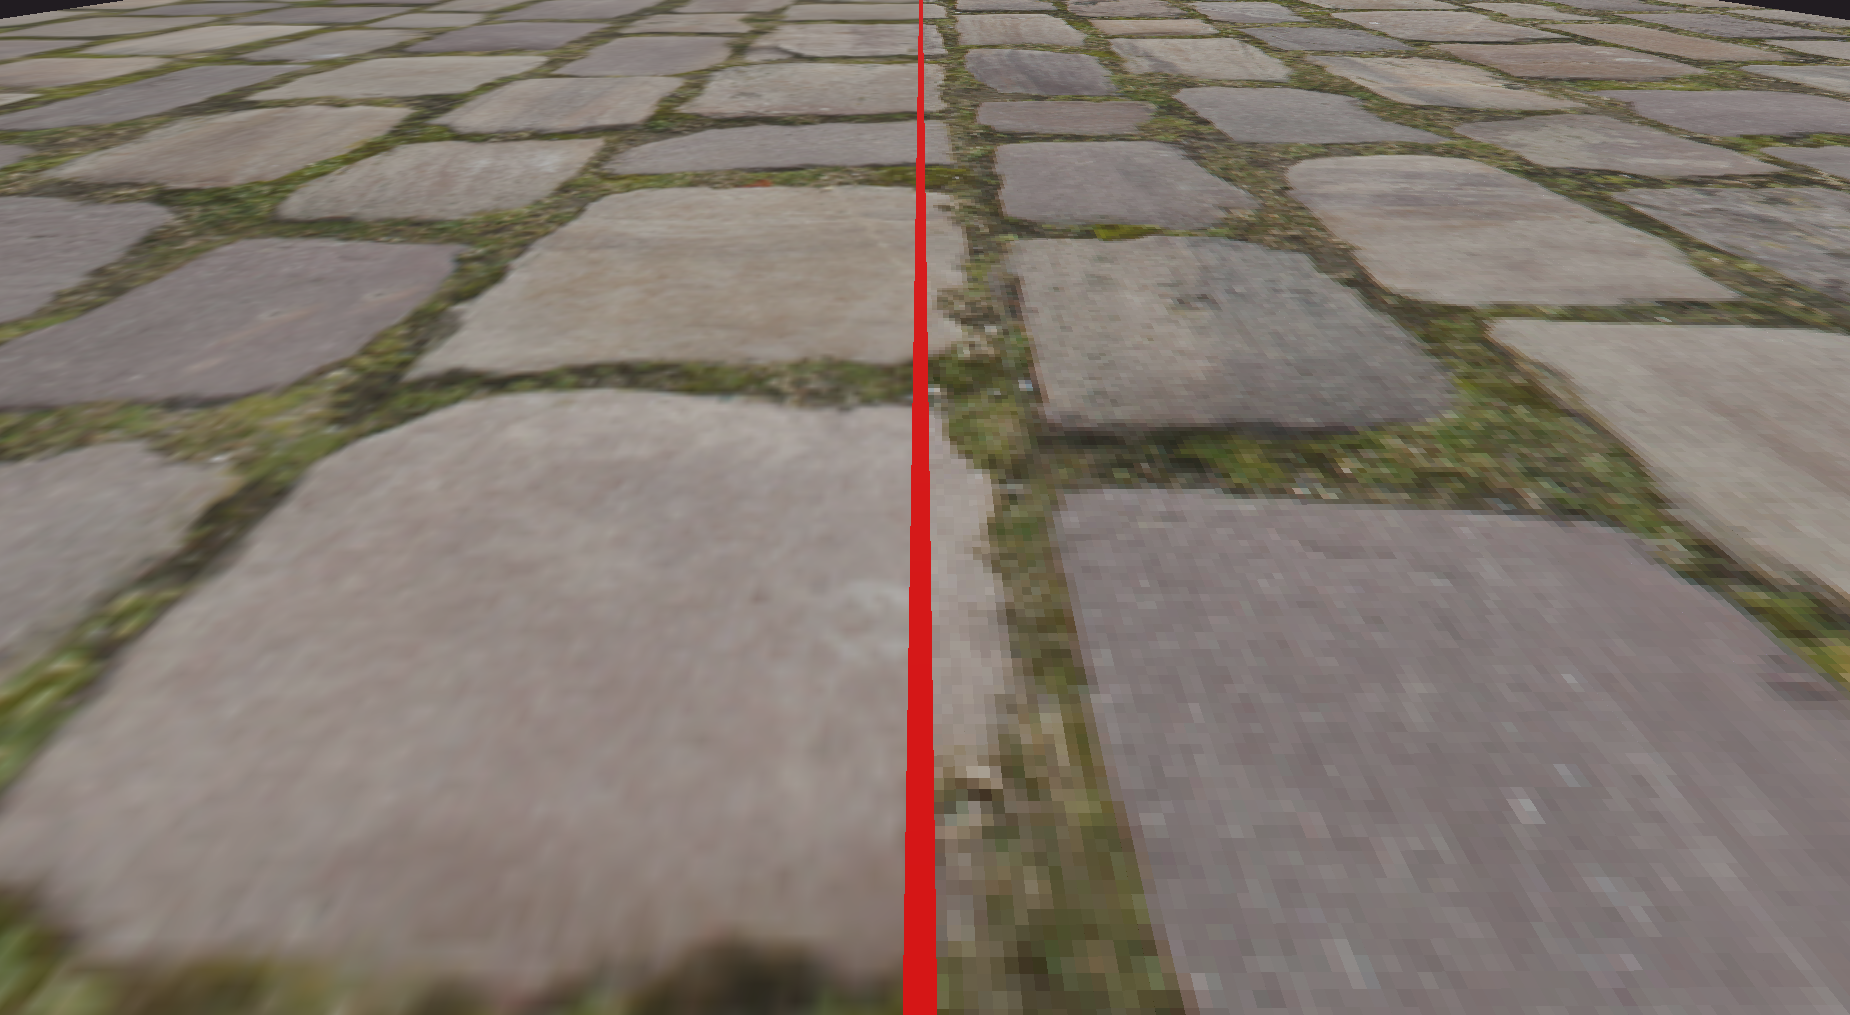
\includegraphics[width=0.9\textwidth]{contenu/resources/images/reconstruction_cpu_vs_gpu}
    \caption[Reconstruction de texture dans \textit{TexSyn}]{Reconstruction de la pyramide de Riesz d'une texture, hors-ligne depuis le CPU (gauche) et en temps-réel depuis le \textit{fragment shader} (droite). On remarque les artefacts de filtrage sur la reconstruction en temps-réel)}
    \label{fig:texsyn-reconstruction}
\end{figure}


\section{Sélection de niveaux de fréquences}

La mise au point de la PC et l'utilisation d'un contexte multi-résolutionnel nous ont permis de visualiser explicitement que les différents niveaux de structure que l'on trouve dans une image sont liés à différents niveaux de d'échelle. Nous avons émis l'hypothèse que chaque niveau de structure que l'on distingue dans une image peut s'exprimer comme la congruence en phases d'un sous-ensemble fréquentiel. Autrement dit, chaque échelle de structure est créée par un sous-ensemble de niveaux de la pyramide d'image. Pour vérifier cela, nous avons regardé quel était le résultat de sélectionner seulement certains sous-ensembles de niveaux de la pyramide et de calculer la PC sur ces niveaux.

\begin{equation}
    PC_{\mathcal{S}}(\mathbf{x}) = \frac{W(x)E(\mathbf{x})}{\epsilon + \sum_{n\in\mathcal{S}} A_{n}(\mathbf{x})},
\end{equation}

où $\mathcal{S}$ est un sous-ensemble de niveaux de la pyramide. En pratique, nous avons essayé avec tous les $\mathcal{S} = \llbracket a, b\rrbracket$ avec $1 \leq a \leq b \leq d$. Cela nous a permit de confirmer que les différents niveaux de structure étaient bien causés par différents sous-ensembles fréquentiels, comme montré à la figure~\ref{fig:pc-selection-niveaux}.

\bigskip

\begin{figure}
    \centering
    \begin{subfigure}[b]{.25\textwidth}
        \centering
        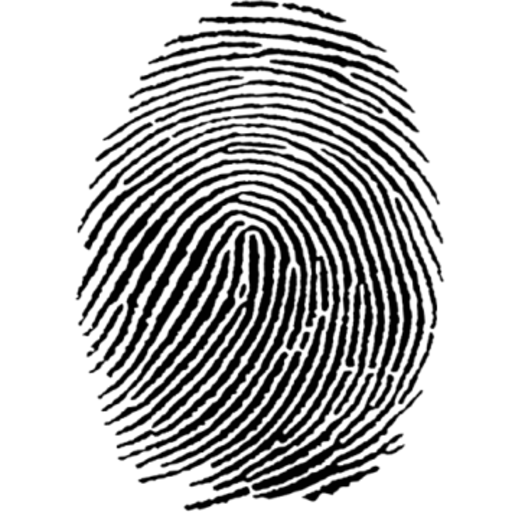
\includegraphics[width=\textwidth]{contenu/resources/images/fingerprint}
        \caption{Image originale}
    \end{subfigure}
    \hfill
    \begin{subfigure}[b]{.25\textwidth}
        \centering
        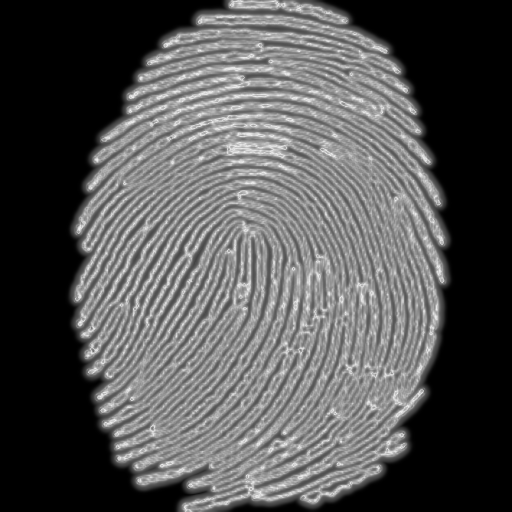
\includegraphics[width=\textwidth]{contenu/resources/images/pc_layer_0_1}
        \caption{Niveaux 0 et 1}
    \end{subfigure}
    \hfill
    \begin{subfigure}[b]{.25\textwidth}
        \centering
        
\includegraphics[width=\textwidth]{contenu/resources/images/pc_layer_2_depth-1}
        \caption{Niveaux 2 à $d-1$}
    \end{subfigure}

    \caption[Congruence de phases sur différents niveaux d'échelle]{Congruence de phases sur différents niveaux d'échelle. Conformément à notre intuition, on observe que sur les premiers niveaux (milieu), qui correspondent aux hautes fréquences, les détails fins ressortent, tandis que sur les derniers niveaux (droite), qui correspondent aux plus basses fréquences, c'est la structure globale, le contour de l'empreinte, qui apparait.}
    \label{fig:pc-selection-niveaux}
\end{figure}

Suite à cette observation, nous avons mis en place une méthode de sélection de niveaux de fréquences, pour pouvoir supprimer certains niveaux de la pyramide et observer l'effet sur la reconstruction. L'objectif était de pouvoir cibler les niveaux de structure qui nous intéressent et les extraire de l'image. Nous avons mis cela en application en faisant du filtrage de bandes de basses fréquences sur des textures de matériaux divers (voir figure~\ref{fig:filter-low-freq}), ce qui nous permet de gommer les tâches présentes sur les images.

\begin{figure}
    \centering
    \begin{subfigure}[b]{.25\textwidth}
        \centering
        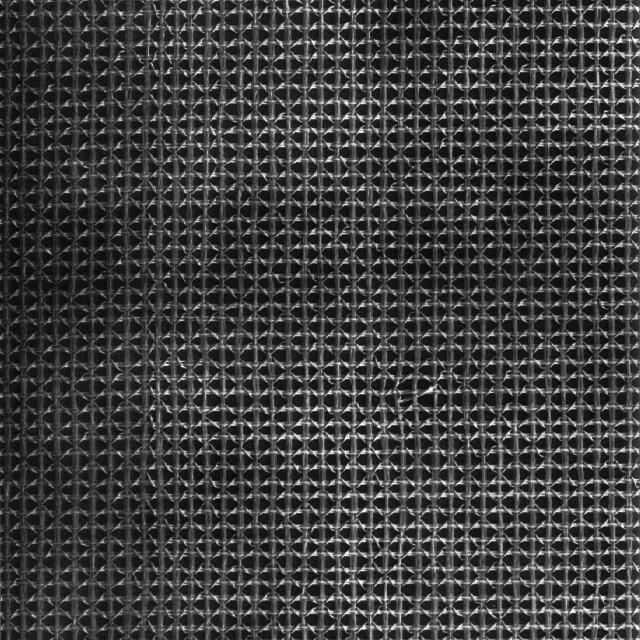
\includegraphics[width=\textwidth]{contenu/resources/images/lattice}
    \end{subfigure}
    \hspace{1em}
    \begin{subfigure}[b]{.25\textwidth}
        \centering
        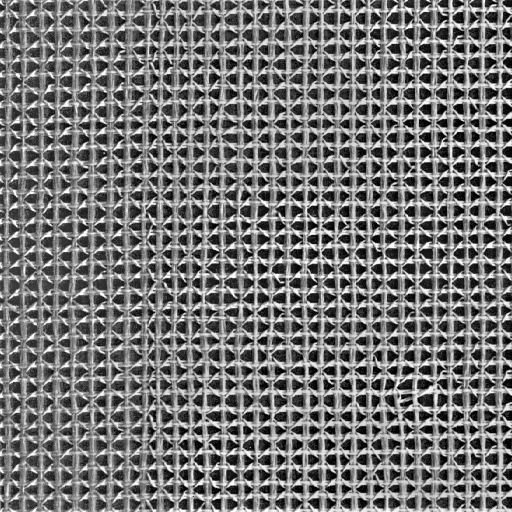
\includegraphics[width=\textwidth]{contenu/resources/images/lattice_filtered}
    \end{subfigure}
    \\
    \vspace{1em}
    \begin{subfigure}[b]{.25\textwidth}
        \centering
        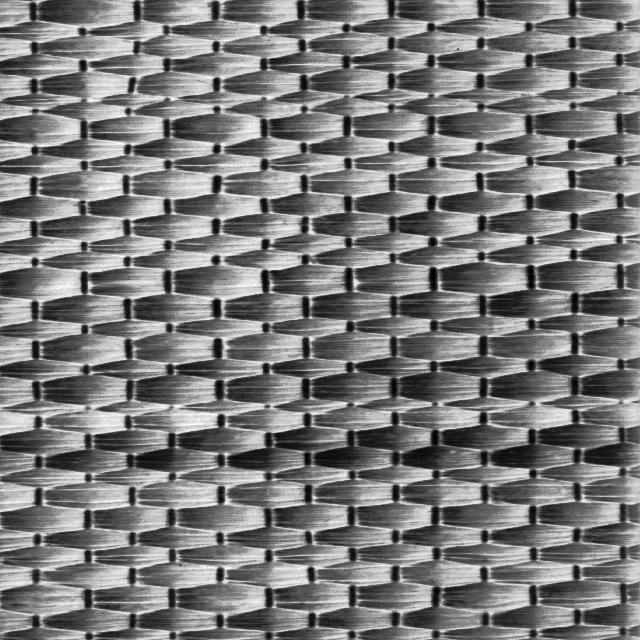
\includegraphics[width=\textwidth]{contenu/resources/images/lattice2}
    \end{subfigure}
    \hspace{1em}
    \begin{subfigure}[b]{.25\textwidth}
        \centering
        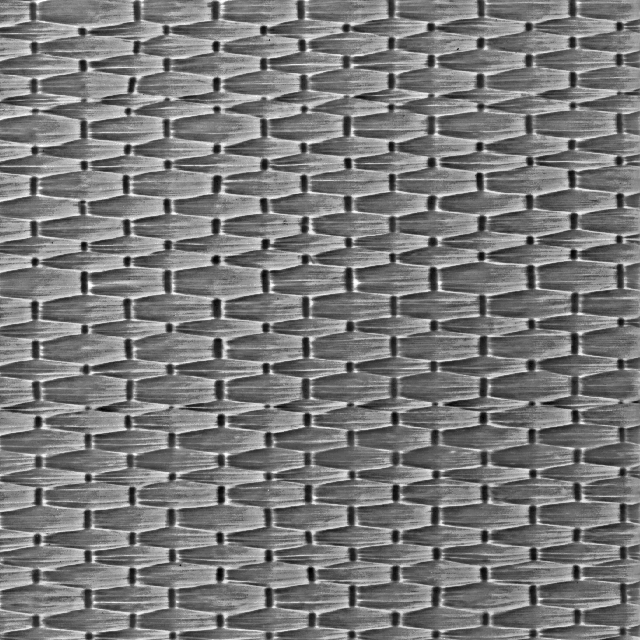
\includegraphics[width=\textwidth]{contenu/resources/images/lattice2_filtered}
    \end{subfigure}

    \caption[Filtrage de bandes de basses fréquences]{Filtrages de bandes de basses fréquences. Cette opération permet de supprimer les tâches présentes sur les textures, tout en conservant la structure globale et les détails. On voit les images originales (gauche) et les images reconstruites sans certains niveaux de la pyramide (droite). On garde typiquement les deux premiers niveaux, ainsi que le dernier, le résidu basse fréquence. Images tirées de la base de textures Brodatz~\cite{abdelmounaime_new_2013}.}
    \label{fig:filter-low-freq}
\end{figure}

\section{Synthèse de texture préservant la congruence de phases}

L'intérêt principal de notre cadre de travail est néanmoins l'utilisation de la PC, notamment en tant qu'indicatrice de la proximité à un bord. La PC se comporte en effet comme un gradient dans la direction perpendiculaire au bord, et nous permet donc de savoir ponctuellement si un pixel se situe proche d'un bord. Nous avons fait quelques expériences pour exploiter ce principe, puis nous avons mis au point une méthode de synthèse de texture pour traiter les textures à structure irrégulière. Nous nous sommes intéressés à un type de textures en particulier, qui présentent des caractéristiques communes. Les textures auxquelles nous nous sommes intéressées, dont quelques exemples sont montrés en figure~\ref{fig:typical-textures}, sont caractérisées par la présence de pavés de toute sorte, entre lesquels se trouve un matériau unique que l'on appelle \og arrière-plan \fg. Ces textures représentent souvent des sols.
% TODO "nous permet de savoir si un pixel se situe proche d'un bord" -> souligner utile pour synthèse en parallèle

\bigskip

\begin{figure}
    \centering
    \begin{subfigure}{.3\textwidth}
        \centering
        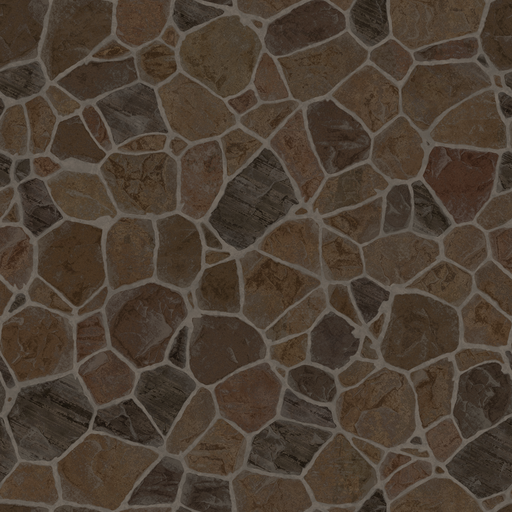
\includegraphics[width=\textwidth]{contenu/resources/images/texture_1}
    \end{subfigure}
    \hfill
    \begin{subfigure}{.3\textwidth}
        \centering
        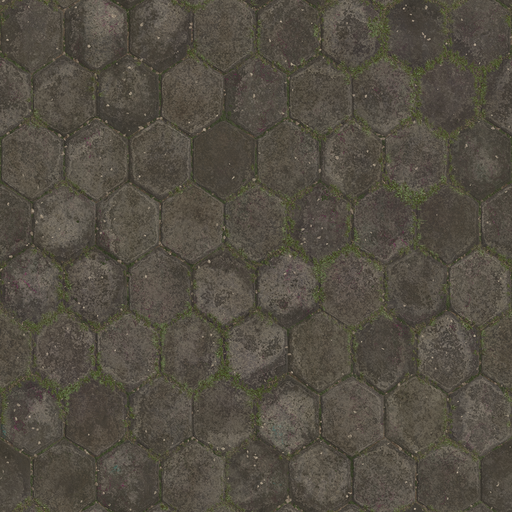
\includegraphics[width=\textwidth]{contenu/resources/images/texture_2}
    \end{subfigure}
    \hfill
    \begin{subfigure}{.3\textwidth}
        \centering
        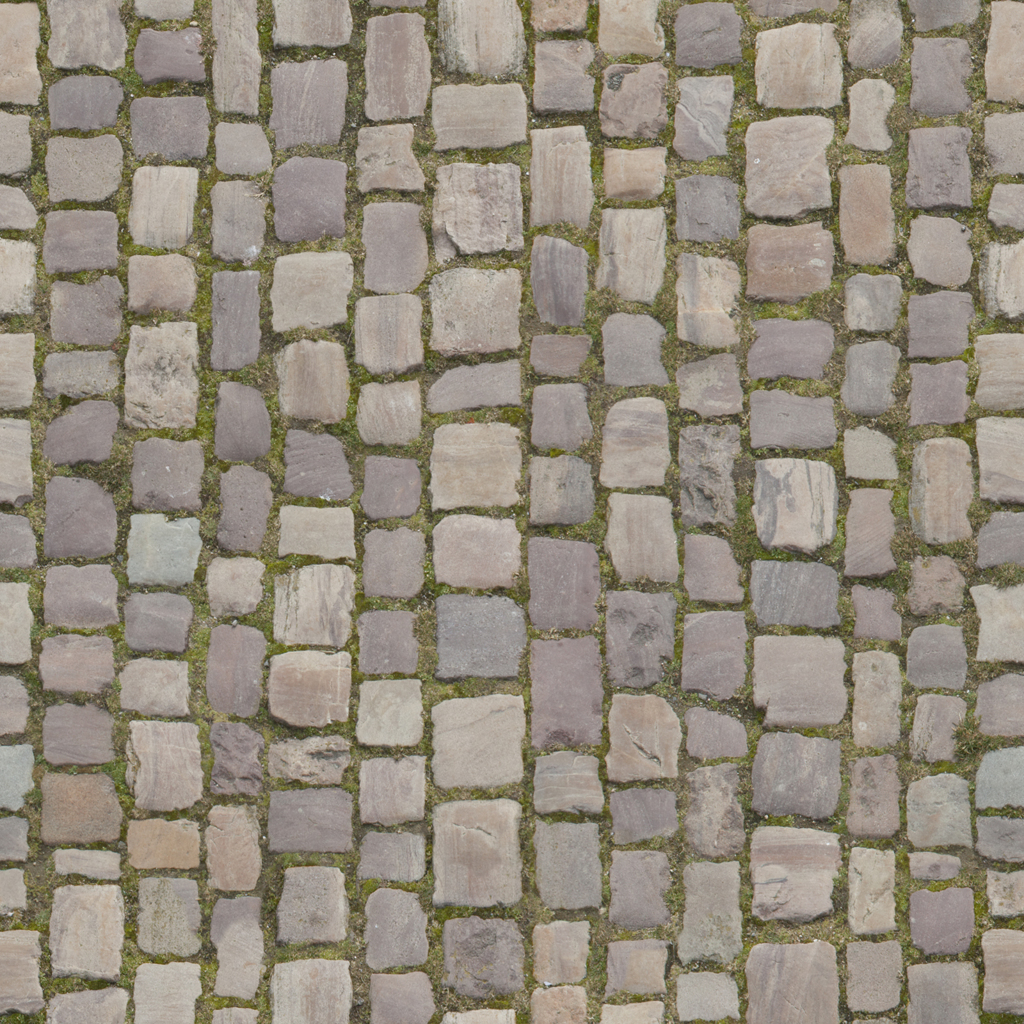
\includegraphics[width=\textwidth]{contenu/resources/images/texture_3}
    \end{subfigure}

    \caption{Exemples du genre de textures à structure irrégulière auquel nous nous sommes intéressés.}
    \label{fig:typical-textures}
\end{figure}


Nous nous sommes inspirés de Lutz et al.~\cite{lutz_preserving_2023}, qui font le constat que les méthodes de synthèse par pavage apériodique, une sorte de synthèse par réorganisation reposant sur un échantillonnage uniforme de l'exemple d'entrée, échouent à préserver la fonction d'autocovariance de l'exemple. Des corrélations qui contribuent à préserver l'apparence de l'entrée sont ainsi mal reproduites, ce qui donne un air trop aléatoire au résultat. Pour remédier à cela, ils améliorent l'étape d'échantillonnage en utilisant le principe d' \og échantillonnage préférentiel \fg{}, qui consiste à influer l'échantillonnage en fonction d'une \og fonction de densité de probabilité \fg{}. En utilisant la fonction d'autocovariance comme densité de probabilité, ils montrent que l'on préserve mieux cette statistique et que l'on améliore la qualité de la synthèse.
%todo cad mal reproduite
% source échantillonnage pref

\bigskip

Nous avons pensé appliquer cette idée à la PC. Nous avons émis l'hypothèse que deux échantillons de contenu provenant d'une même composante, avec une PC similaire, ont un profil de couleurs similaire, puisqu'ils se situent à une même distance d'un bord. Pour vérifier cela, nous avons mis au point une méthode de synthèse qui préserve la PC de l'exemple. Le principe de la synthèse que nous proposons est de réorganiser le contenu de l'exemple à l'aide d'un échantillonneur qui nous indique, à chaque endroit, un remplacement possible. Cet échantillonneur prend en compte l'endroit où l'on se situe dans la texture pour trouver un contenu de remplacement idéal et créer de la nouveauté. Différentes propriétés sont prises en considération pour calculer cette indirection, notamment la PC. Les étapes de cette méthode sont détaillées dans la section qui suit.

\bigskip

Pour notre application, nous avons décidé de travailler avec le contenu le plus petit possible pour notre réorganisation : le pixel. Bien qu'il y ait des avantages à travailler avec des petites régions de pixels plutôt que des pixels unitaires, et que de nombreuses méthodes de la littérature font ce choix~\cite{wei_state_2009}, nous avons décidé de travailler avec des pixels pour avoir un premier prototype rapide et pouvoir tester notre hypothèse. L'utilisation de l'échantillonneur s'adapte en effet particulièrement bien à l'échelle du pixel, contrairement à la synthèse par patch, qui demande plus d'efforts de mise en place.

\subsection{Échantillonneur préservant la congruence de phases}

Pour mettre en place notre échantillonneur, on reprend la stratégie proposée par Pharr et al. dans leur livre~\cite{pharr_physically_2023}, qui utilise la méthode de la transformée inverse. Cette méthode d'échantillonnage repose sur le fait que pour échantillonner une variable aléatoire de loi donnée, il suffit d'échantillonner une variable aléatoire uniforme et d'appliquer la fonction de répartition inverse de la loi. Pour appliquer cette méthode, on commence par définir l'échantillonnage d'une fonction constante par morceaux 1D. Pour une fonction $f$ constante par morceaux :


\begin{equation}
    f(x) = \left\{
        \begin{array}{ll}
            v_0 & \mbox{si } x \in [x_0, x_1] \\
            v_1 & \mbox{si } x \in [x_1, x_2] \\
            \vdots & \vdots \\
            v_{N-1} & \mbox{si } x \in [x_{N-1}, x_N]
        \end{array}
    \right.
\end{equation}

d'intégrale $I$ :

\begin{equation}
    I = \int_{0}^{1} f(x) dx = \sum_{i=0}^{N-1} \frac{v_i}N,
\end{equation}

si on considère (sans perte de généralité) que $f$ est définie entre 0 et 1, et que les $x_i$ sont disposés de manière régulière $x_i = i / N$. La fonction de densité de probabilité associée à $f$ est alors simplement $p(x) = f(x) / I$. La fonction de répartition $F$ est linéaire par morceaux, définie aux $x_i$ :

\begin{equation}
    F(x_i) = \int_{0}^{x_i} p(t) dt = \sum_{j=0}^{x_i} \frac{v_j}{NI} = F(x_i-1) + \frac{v_i-1}{NI},
\end{equation}

et de coefficient directeur $v_i/I$ entre $x_i$ et $x_{i+1}$. On peut échantillonner $f$ en échantillonnant une variable aléatoire uniforme $u$ et en calculant $F^{-1}(u)$.

\bigskip

% TODONT finish diagram perhaps, to show inversion method on 1D piecewise constant function
%\begin{tikzpicture}
%    \begin{axis}[
%        title={Fonction de répartition},
%        symbolic x coords={$x_0$, $x_1$, $x_2$, $x_3$},
%        ybar stacked,
%        ytick={0, 1}
%    ]
%        \addplot coordinates {
%            (x_0,0.3) (x_1,0.3) (x_2,0.3) (x_3,0.3)
%        };
%        \addplot coordinates {
%            (x_1, 0.2) (x_2, 0.2) (x_3, 0.2)
%        };
%        \addplot coordinates {
%            (x_2, 0.4) (x_3, 0.4)
%        };
%        \addplot coordinates {
%            (x_3, .1)
%        };
%
%        \node [above] at (0, 0.15) {$p_1$};
%        \node [above] at (1, 0.15) {$p_1$};
%        \node [above] at (0, 0.15) {$p_1$};
%        \node [above] at (0, 0.15) {$p_1$};
%
%    \end{axis}
%
%\end{tikzpicture}

% TODO Il suffit
Il suffit ensuite de constater que nos textures sont des tableaux, donc des fonctions constantes par morceaux 2D, et que leur loi de probabilité conditionnelle et marginale sont des fonctions constantes par morceaux 1D. La stratégie est ainsi d'échantillonner la probabilité marginale pour avoir la première coordonnée, puis d'échantillonner la probabilité conditionnelle en utilisant la première valeur trouvée pour déterminer la deuxième coordonnée.

\subsection{Synthèse avec l'échantillonneur préférentiel}

On va maintenant utiliser ce principe d'échantillonnage préférentiel pour synthétiser du nouveau contenu, en préservant la fonction de PC. Pour cela, on veut pour chaque pixel tirer un nouveau pixel, avec une PC similaire. On souhaiterait avoir une fonction de densité de probabilité adaptée pour chaque valeur de PC, qui privilégie l'échantillonnage des valeurs autour de $x$ pour tout $x$ dans l'espace des valeurs de la PC, $[0, 1]$. Cependant, la PC est à valeurs continues, il serait trop compliqué de stocker une fonction de densité pour chaque valeur. Pour résoudre ce problème, la PC est quantifiée en $N$ intervalles de taille constante $1/N$ de telle sorte que l'intervalle $i$ soit juste les valeurs de la PC entre $[i/N, (i+1)/N[$. Ce sont ces intervalles qui nous servent de densité de probabilité pour l'échantillonnage préférentiel. En pratique, on utilise $N=10$ et on partitionne en fait entre les valeurs minimum et maximum de la PC calculée, plutôt qu'entre 0 et 1, qui sont les extremums théoriques. Au moment de tirer du nouveau contenu, on regarde la valeur de PC du pixel que l'on cherche à remplacer, et on échantillonne avec la densité de probabilité correspondant à l'intervalle de PC dans lequel il se trouve.

\bigskip

Pour préserver la cohérence dans l'image, on fait aussi attention à ne pas mélanger les contenus provenant de différentes \og composantes \fg de notre image. Les images auxquelles nous nous intéressons ont souvent deux composantes, les pavés et l'arrière-plan. On partitionne donc notre image entre les différentes composantes à l'aide d'une classification par l'algorithme des K-moyennes. On obtient ainsi un masque binaire pour chaque composante, que l'on applique sur les intervalles de PC par multiplication, pour obtenir la densité de probabilité finale, pour chaque composante et chaque niveau de PC.

\bigskip

Pour utiliser efficacement notre échantillonneur dans la synthèse en temps-réel, on a d'abord une première étape de pré-calcule hors-ligne, où l'on calcule plusieurs réalisations de l'échantillonneur, pour chaque composante et pour chaque intervalle de PC, afin d'augmenter la variété de l'échantillonneur. Ces réalisations sont des vecteurs de translations $(u, v)$, que l'on stocke dans une carte de texture pour les charger sur le GPU. Cette texture est un jeu de données à trois dimensions : une pour les subdivisions de la PC, une pour les différentes composantes et la dernière pour les différentes réalisations de l'échantillonneur. Un schéma explicatif est montré à la figure~\ref{fig:sampler-realization}.

\begin{figure}
    \centering
    \begin{subfigure}{.5\textwidth}
        \centering
        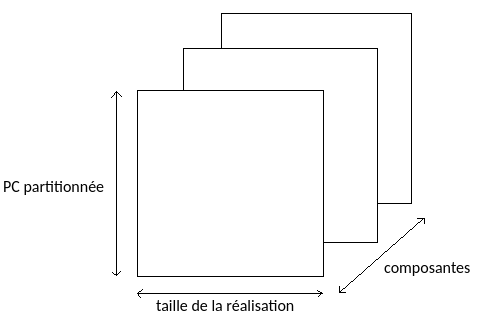
\includegraphics[width=\textwidth]{contenu/resources/images/sampler_realization}
    \end{subfigure}
    \hfill
    \begin{subfigure}{.45\textwidth}
        \centering
        
\includegraphics[width=\textwidth]{contenu/resources/images/realization_pc_0}
    \end{subfigure}

    \caption[Réalisation de l'échantillonneur préférentiel]{Schéma explicatif de la texture 3D où on stocke la réalisation de l'échantillonneur (gauche) et un exemple de réalisation pour une composante avec 10 niveaux de subdivisions de PC, et 128 échantillons (droite).}
    \label{fig:sampler-realization}
\end{figure}

On utilise ensuite cette texture dans le \textit{fragment shader} lors du rendu pour faire l'échantillonnage en temps-réel. On observe la valeur de PC et la composante du pixel que l'on cherche à remplacer, pour aller chercher la bonne réalisation dans la texture 3D. On choisit ensuite aléatoirement entre les réalisations qui ont la même PC et la même composante. En pratique, cela se fait à l'aide d'une fonction de hachage, avec les coordonnées $(u, v)$ du fragment pour lequel on échantillonne.

\bigskip

\begin{figure}
    \centering
    \begin{subfigure}{.95\textwidth}
        \centering
        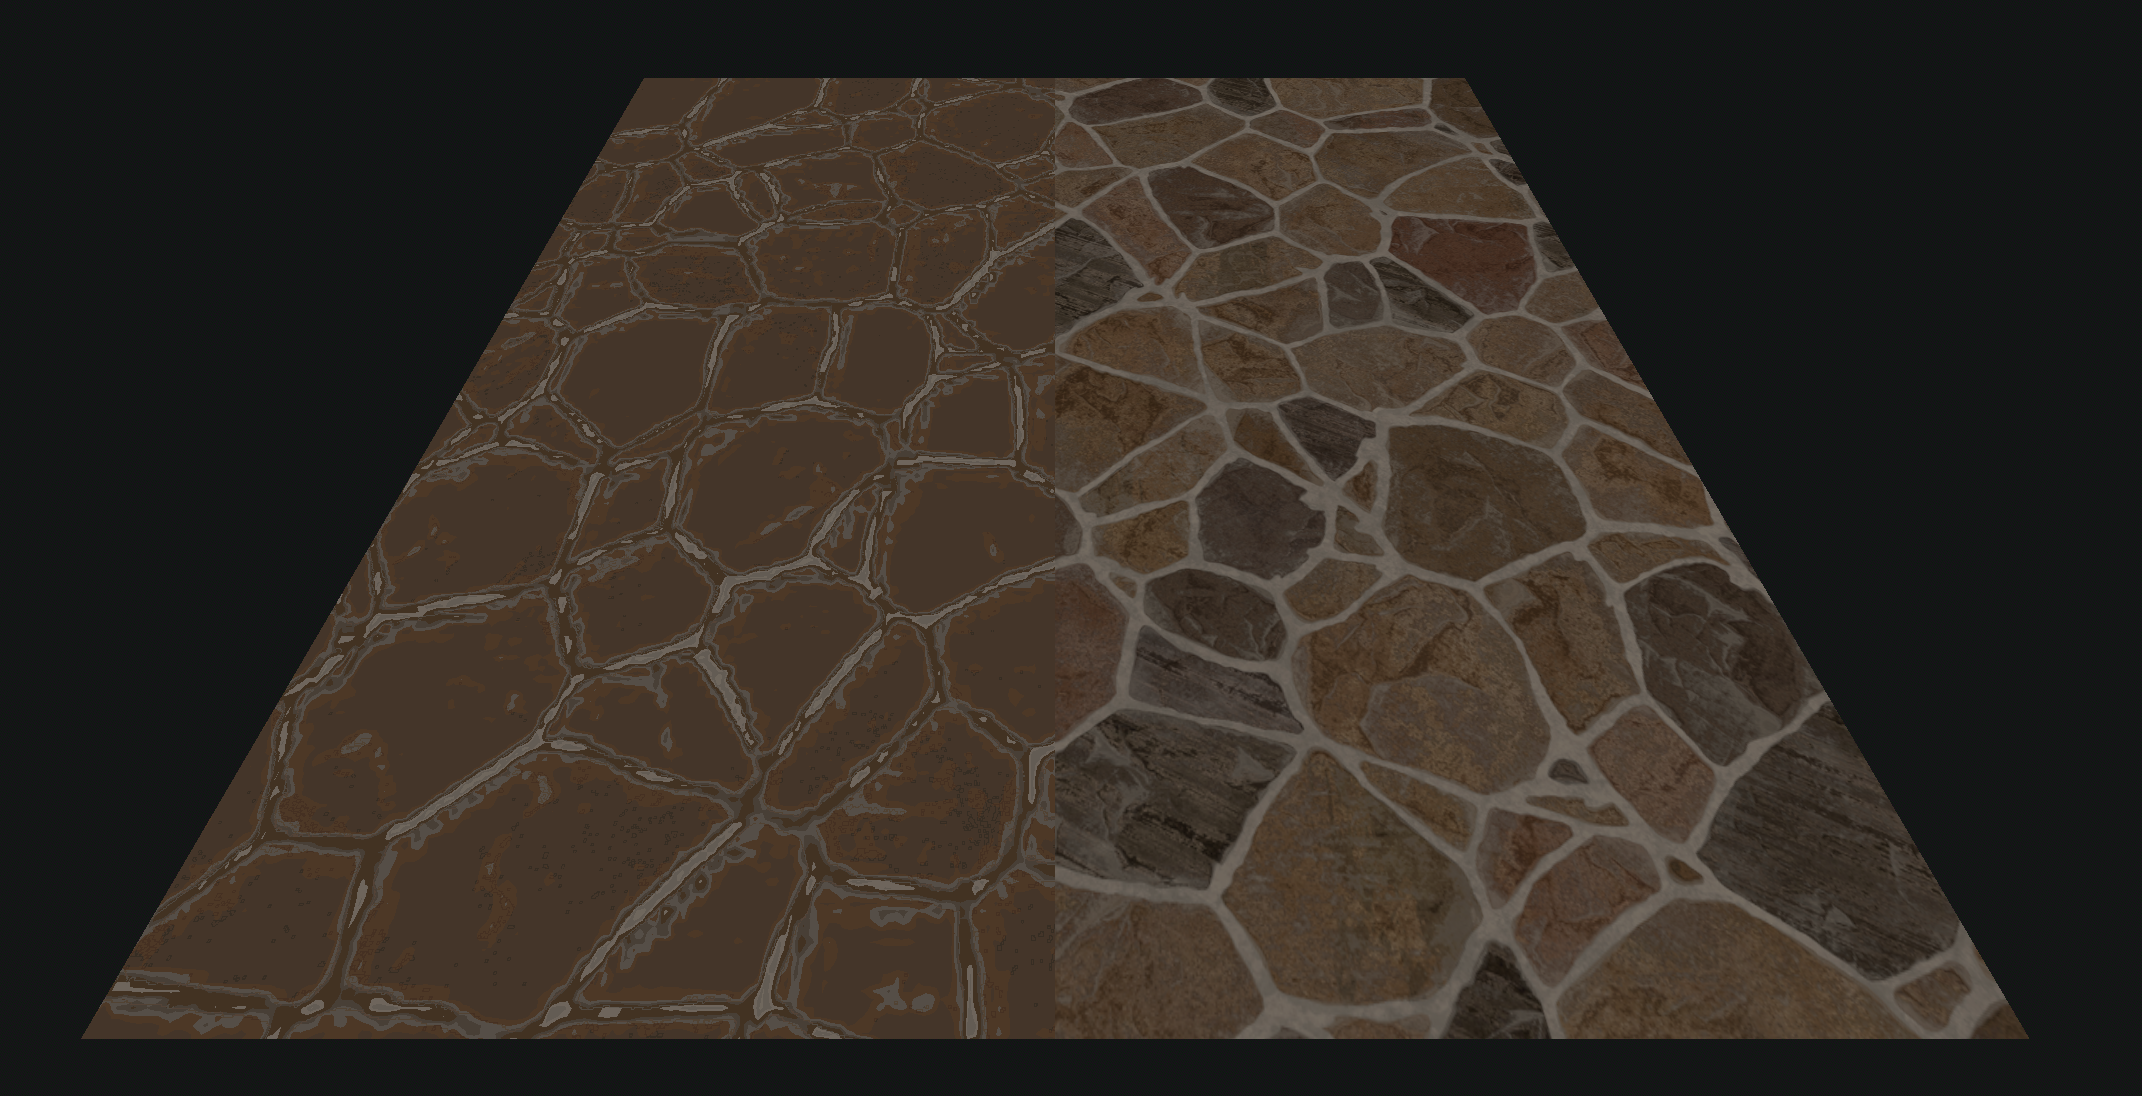
\includegraphics[width=\textwidth]{contenu/resources/images/partitioned_sampling_pc_preserving_no_shuffle}
    \end{subfigure}
    \\
    \begin{subfigure}{.95\textwidth}
        \centering
        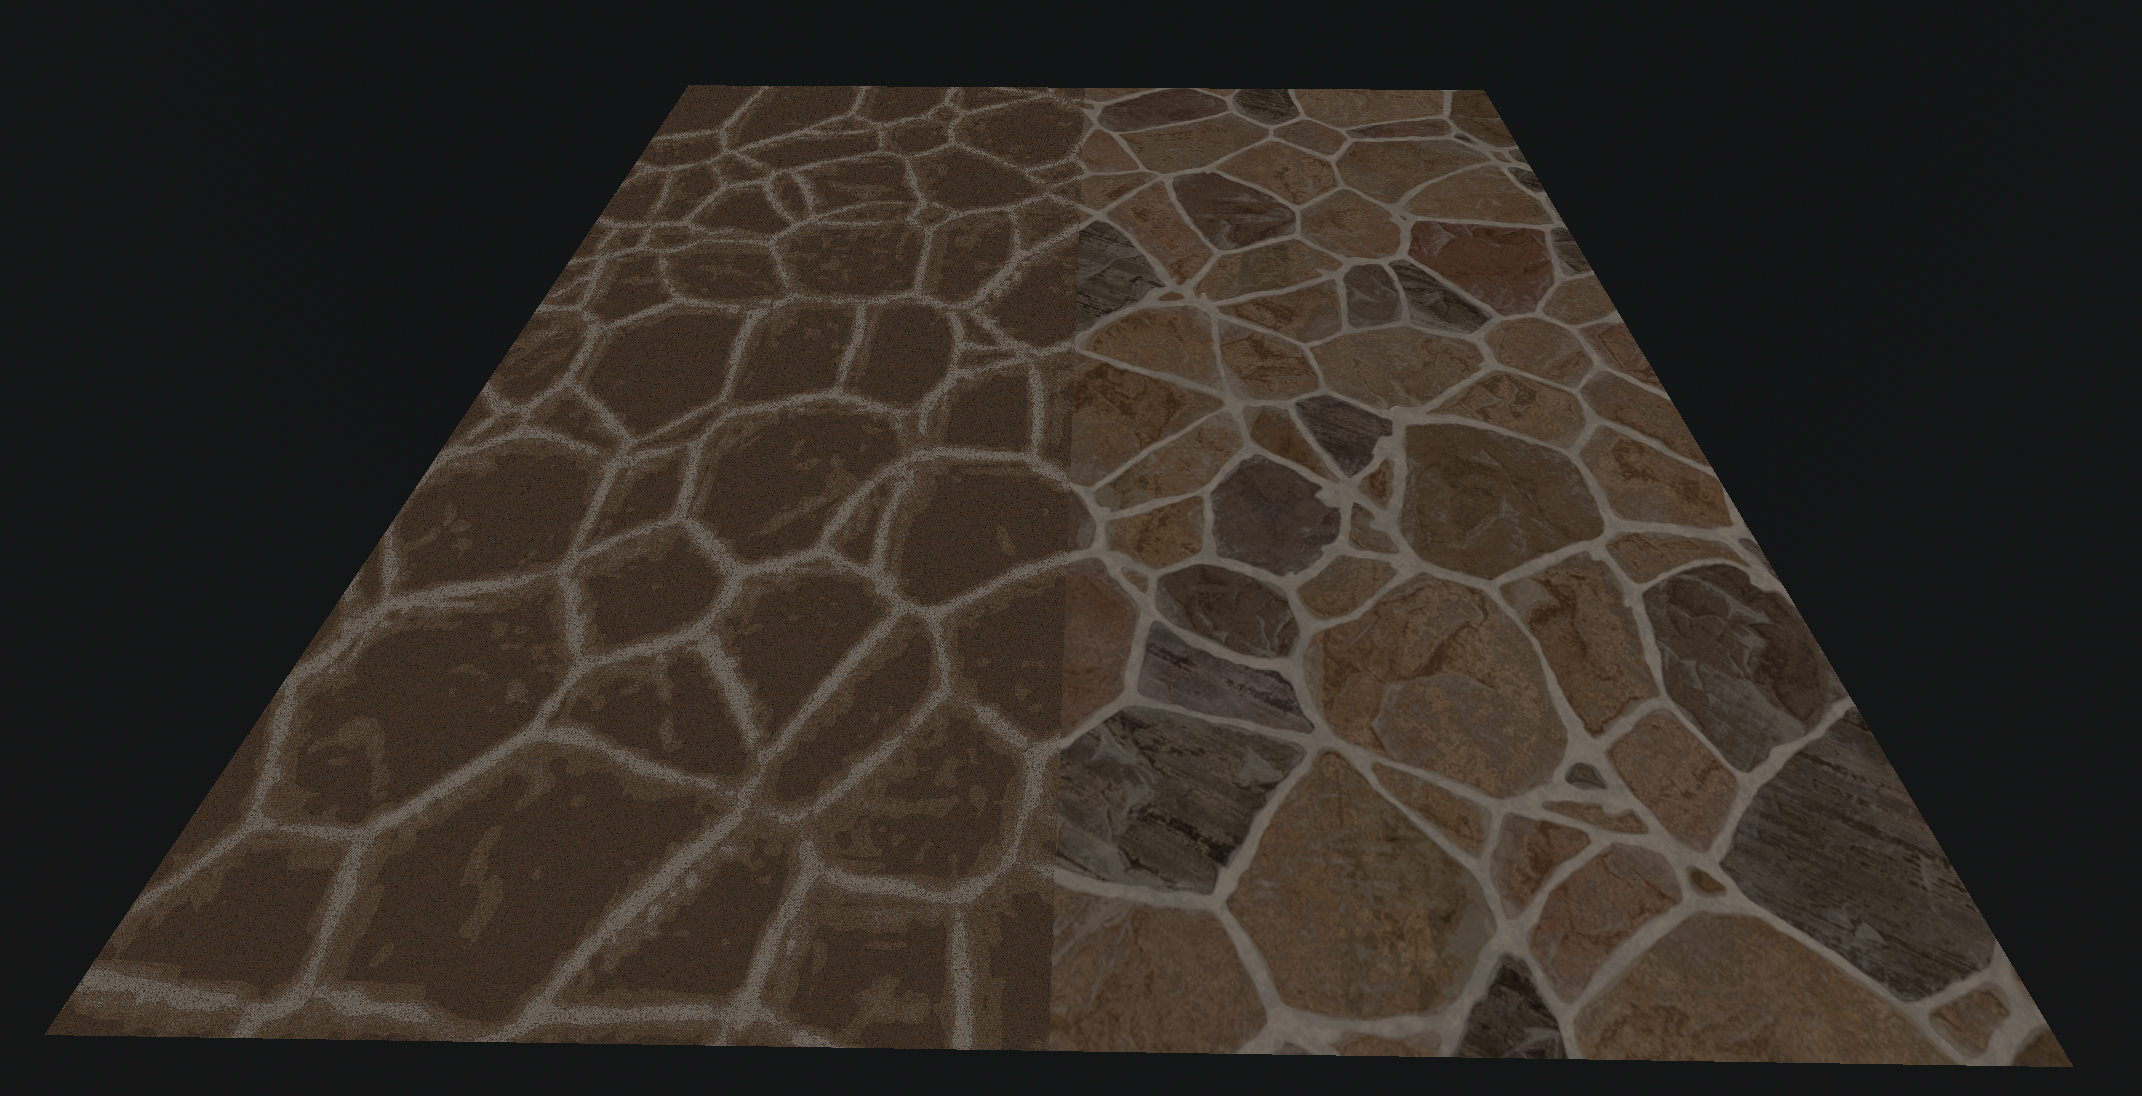
\includegraphics[width=\textwidth]{contenu/resources/images/partitioned_sampling_pc_preserving_shuffle_uv}
    \end{subfigure}
    \caption[Échantillonnage avec et sans multiples réalisations]{Comparaison du résultat de l'échantillonnage avec et sans multiples réalisations. La partie de droite de chaque image montre la texture originale. On voit que l'échantillonnage avec une seule réalisation (haut) donne le même échantillonnage pour plusieurs pixels, tandis qu'utiliser plusieurs réalisations (bas) apporte de la variété.}
    \label{fig:offset-shuffle}
\end{figure}

Pour savoir quel pixel remplacer lorsque l'on évalue notre \textit{fragment shader}, on utilise le pavage périodique. On duplique et on translate l'exemple d'entrée pour couvrir la surface à remplir. On utilise alors les coordonnées de texture du fragment pour savoir quel pixel de l'exemple d'entrée aller chercher. On peut ainsi calculer la PC de l'exemple d'entrée, et l'utiliser pour échantillonner le nouveau contenu. Le pavage périodique est connu pour créer des artefacts visuels, notamment des motifs de répétition. Cependant, nous pensons que l'utilisation de l'échantillonneur pourra atténuer ces artefacts, en apportant de la variété dans l'échantillonnage.

\begin{figure}[t]
    \centering
    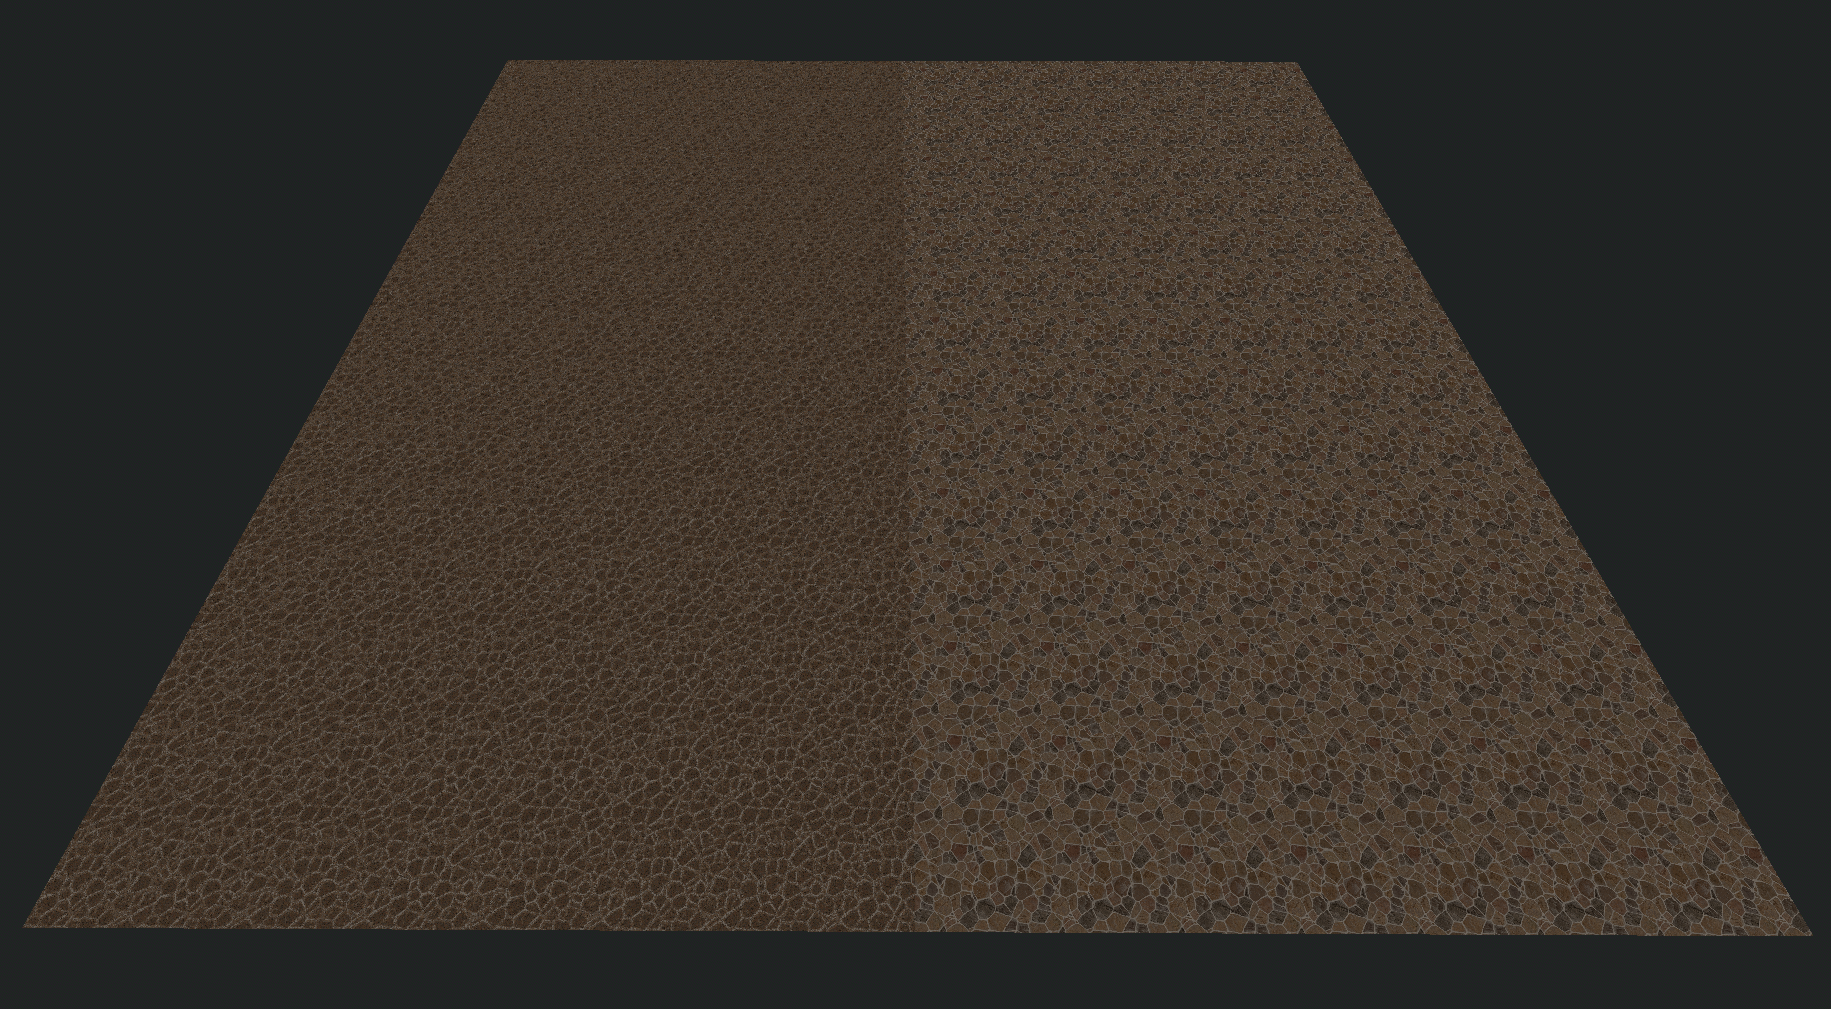
\includegraphics[width=\textwidth]{contenu/resources/images/partitioned_sampling_pc_preserving_shuffle_uv_far}
    \caption[Résultat de l'échantillonnage avec multiples réalisations, vu de loin.]{Résultat de l'échantillonnage avec multiples réalisations, vu de loin. On remarque que l'échantillonnage préférentiel permet d'atténuer les artefacts visuels dûs à la répétition du pavage périodique. La partie droite de la surface est recouverte par un pavage périodique classique.}
    \label{fig:pc-preserving-synthesis}
\end{figure}

\section{Discussion}

Dans ce chapitre, nous avons présenté plusieurs applications de la PC d'une image, à savoir la sélection de niveaux de fréquences et la synthèse de texture préservant la structure. Nous présentons ici une analyse des résultats obtenus et discutons RE des observations que l'on peut retenir et des limites de notre approche.

\paragraph{Sélection de niveaux de fréquences}

La sélection de niveaux de fréquences par l'élimination de niveaux de la pyramide d'image est une méthode qui permet de visualiser différentes échelles de structure présentes dans l'image. Les différents niveaux de structure que l'on distingue dans une image sont liés à certaines fréquences dans le domaine spectral, et donc à différents niveaux de la pyramide d'image. Étudier et sélectionner différents niveaux de la pyramide permet de mieux comprendre la structure de l'image. Nous avons mis à profit la sélection de niveaux en faisant du filtrage de bandes de basses fréquences pour effacer des \og tâches \fg présentes sur des textures comme présenté en figure~\ref{fig:filter-low-freq}. Une méthode similaire a d'ailleurs été publiée~\cite{zhang_pyramid_2023} indépendamment de nous, au cours des derniers mois de ce travail. Nous n'avons pas fait la comparaison des deux méthodes, car ce n'était pas le but de cette recherche.

\bigskip

Le processus présente cependant des désavantages. D'abord, il relève d'un travail manuel, où l'utilisateur doit lui-même observer les congruences de phases partielles, qui ne comportent pas tous les étages de la pyramide, et décider lesquels supprimer ou garder. La tâche peut être fastidieuse et manque de métrique de décision pour automatiser et homogénéiser la démarche. De plus, la méthode souffre du problème que les bandes de fréquences parasites sont parfois corrélées à du contenu que l'il serait souhaitable de préserver de mêmes fréquences. Il est alors impossible avec cette méthode d'ôter précisément le contenu indésirable, sans affecter le reste de la texture.
% TODO que l'il whack
\paragraph{Synthèse de texture préservant la congruence de phases}
\label{par:discussion-synthesis}

La synthèse de texture préservant la PC est la deuxième application de la PC et est au cœur de ce travail. C'est un prototype de recherche mis au point pour examiner l'hypothèse que la PC, qui est un indicateur de la proximité d'un bord, donne aussi une mesure de ressemblance entre plusieurs contenus d'une texture. Cette méthode RE n'a pas donné lieu à une synthèse utilisable, mais elle a mené à plusieurs observations sur l'utilisation de la PC appliquée au domaine de la synthèse de texture.

\bigskip

% TODO il est clair
Tout d'abord, il est clair au vu des résultats montrés en figure~\ref{fig:pc-preserving-synthesis} que la PC seule ne suffit pas à capturer la similarité entre deux contenus. On remarque sur la figure que la couleur des pavés reconstruits tend vers un marron qui semble être la moyenne des couleurs des pavés de l'image. En effet, cette méthode d'échantillonnage ne prend pas en compte la couleur de chaque pavé et échantillonne sans distinction dans des pavés de couleurs différentes. Même si la PC est préservée, la couleur est mélangée et on perd en variété.
% TODO partie sur la moyenne, mieux epliquer / justifier

\bigskip

La PC semble cependant bien détecter et, dans une certaine mesure préserver, des éléments de structure internes aux pavés. On voit à la figure~\ref{fig:mark-preserved} que les marques ou fissures dans les pavés sont encore présentes après la synthèse. Cette caractéristique a néanmoins un désavantage : l'échantillonneur ne fait pas de distinction entre le bord d'un pavé et le bord d'une marque à l'intérieur d'un pavé, comme montré à la figure~\ref{fig:pc-defect}. Des pixels sont donc échantillonnés au mauvais endroit et le contenu des bords et des marques des pavés sont mélangés, ce qui n'est pas désirable.

\bigskip

\begin{figure}
    \centering
    \begin{subfigure}{.45\textwidth}
        \centering
        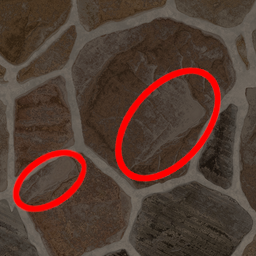
\includegraphics[width=\textwidth]{contenu/resources/images/marks}
    \end{subfigure}
    \hfill
    \begin{subfigure}{.45\textwidth}
        \centering
        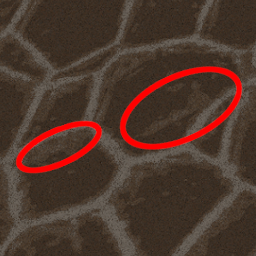
\includegraphics[width=\textwidth]{contenu/resources/images/mark_preserved}
    \end{subfigure}

    \caption[L'échantillonneur préserve partiellement les marques dans les pavés]{Zoom sur deux marques présentes au sein d'un pavé de la texture (gauche) qui se retrouvent sur la texture synthétisée avec notre échantillonneur (droite). }
    \label{fig:mark-preserved}
\end{figure}

\begin{figure}
    \centering
    \begin{subfigure}{.45\textwidth}
        \centering
        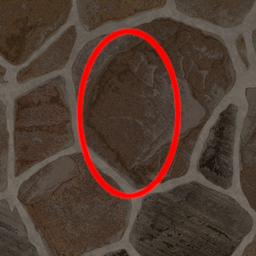
\includegraphics[width=\textwidth]{contenu/resources/images/stone_zoom}
    \end{subfigure}
    \hfill
    \begin{subfigure}{.45\textwidth}
        \centering
        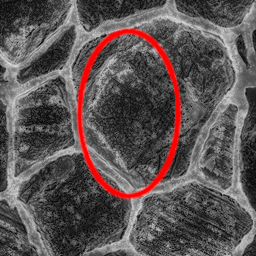
\includegraphics[width=\textwidth]{contenu/resources/images/stone_zoom_pc}
    \end{subfigure}

    \caption[Problème d'échantillonnage dû à la présence de marques au sein des pavés de la texture]{Zoom sur une marque présente au sein d'un pavé de la texture (gauche) et la PC associée à cette zone (droite). La PC a des valeurs semblables sur les bords du pavé et autour de la marque foncée mise en évidence. Cela cause des problème pour l'échantillonnage.}
    \label{fig:pc-defect}
\end{figure}

Le mélange des couleurs que l'on observe est aussi dû à notre choix de travailler avec des pixels unitaires plutôt que des petites régions de pixels. La préservation de la PC à elle seule n'est pas suffisante pour préserver des corrélations locales, comme la couleur, quand on agit au niveau du pixel. Il faudrait travailler avec des régions de pixels pour avoir du contenu moins décorrélé de son entourage ou trouver une manière d'accorder une plus grande importance au voisinage local lorsque l'on échantillonne du nouveau contenu.

\bigskip

Enfin une dernière observation est que la synthèse gagnerait en variété si une disposition des pixels autre qu'un pavage périodique était utilisée. Ce choix a été fait pour des questions de simplicité, car le sujet de l'étude était l'échantillonneur plus que la disposition. L'utilisation de l'échantillonneur permet d'atténuer les artefacts visuels dûs à la répétition du pavage périodique, mais ces derniers sont encore visibles quand on regarde de loin, comme à la figure~\ref{fig:pc-preserving-synthesis}. La recherche de méthode d'organisation de contenu pour générer des nouvelles dispositions (par exemple des pavés de forme similaire, mais différente à tous les autres pavés de l'exemple) en temps réel est cependant un sujet difficile et est encore ouvert aujourd'hui~\cite{guehl_semi-procedural_2020, baldi_differentiable_2023}.